Este capítulo aborda o planejamento, execução e análise do método proposto por este trabalho, a fim de verificar a viabilidade do projeto, bem como sua eficiência. O sistema computacional desenvolvido denomina-se \productname{} e tem seu código-fonte disponível em \url{https://github.com/rodrigost23/automailx}.

%==========================================================================
%
\section{Planejamento dos experimentos}\label{sec:result_planejamento}
%
%==========================================================================

O intuito desta avaliação experimental é verificar a capacidade do sistema \productname{} de classificar as ações do usuário a partir da leitura de sensores, e exibir um modelo virtual animado que demonstra os dados lidos e a detecção dos movimentos realizados. Neste sentido, foram definidas as seguintes questões de pesquisa:

\begin{enumerate}[label=\textbf{QP\arabic*:}, ref=QP\arabic*]
	\item O sistema \productname{} é capaz de replicar os movimentos realizados pelo usuário em um ambiente virtual?\label{qp:simula_movimentos}
	\item A previsão de movimentos do sistema \productname{} é precisa o suficiente para garantir a sua confiabilidade?\label{qp:acuracia}
	\item O sistema \productname{} pode prever as ações da prótese virtual em tempo real a partir dos dados dos sensores?\label{qp:previsao_sensores}
	      % \item O sistema \productname{} tem desempenho consistente independente do usuário?\label{qp:usuarios_diferentes}
\end{enumerate}

Visando responder essas questões, foi definido um ambiente que consiste em um sistema de captura de movimentos acoplado ao \textit{software} simulador sendo executado em um computador.
% 
% \subsection{Captura dos movimentos}\label{sec:result_captura}
% 
O protótipo para captura de dados consiste em um módulo GY\=/\(521\) com um sensor MPU-\(6050\)~\cite{invensense:imu_mpu}, que contém um acelerômetro e um giroscópio, e um sensor flexível SparkFun de \(2{,}2\) polegadas~\cite{flex:datasheet}, conectados em um Arduino Nano 3.0 conforme o esquema da \autoref{fig:result_schem}.

\begin{figure}[ht]
	\caption{\label{fig:result_schem}Esquema das conexões dos sensores ao Arduino}
	\begin{center}
		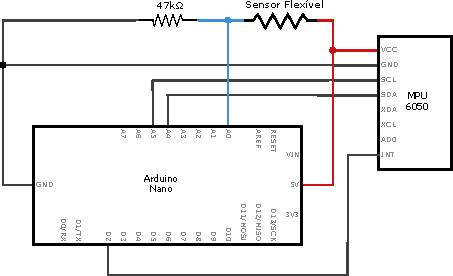
\includegraphics[width=.8\textwidth]{resources/result_schem}
	\end{center}
	\legend{Fonte: Elaborada pelo autor}
\end{figure}

Todos esses equipamentos foram fixados em uma joelheira de material flexível não rígido, como visto na \autoref{fig:result_prototipo}, com o MPU\=/\(6050\) (a) posicionado acima do joelho, e o sensor flexível (b) posicionado na parte de trás. Este último sensor teve de ser posicionado desta forma devido ao seu comprimento de apenas \SI{55.88}{\milli\meter}, já que posicionamento na parte frontal do joelho, como planejado na ~\autoref{sec:metodo_protese}, impediria que a resistência do sensor variasse o suficiente.

\begin{figure}[ht]
	\caption{\label{fig:result_prototipo}Joelheira com o Arduino Nano, o MPU-6050 (a) e o sensor flexível (b) fixados}
	\begin{center}
		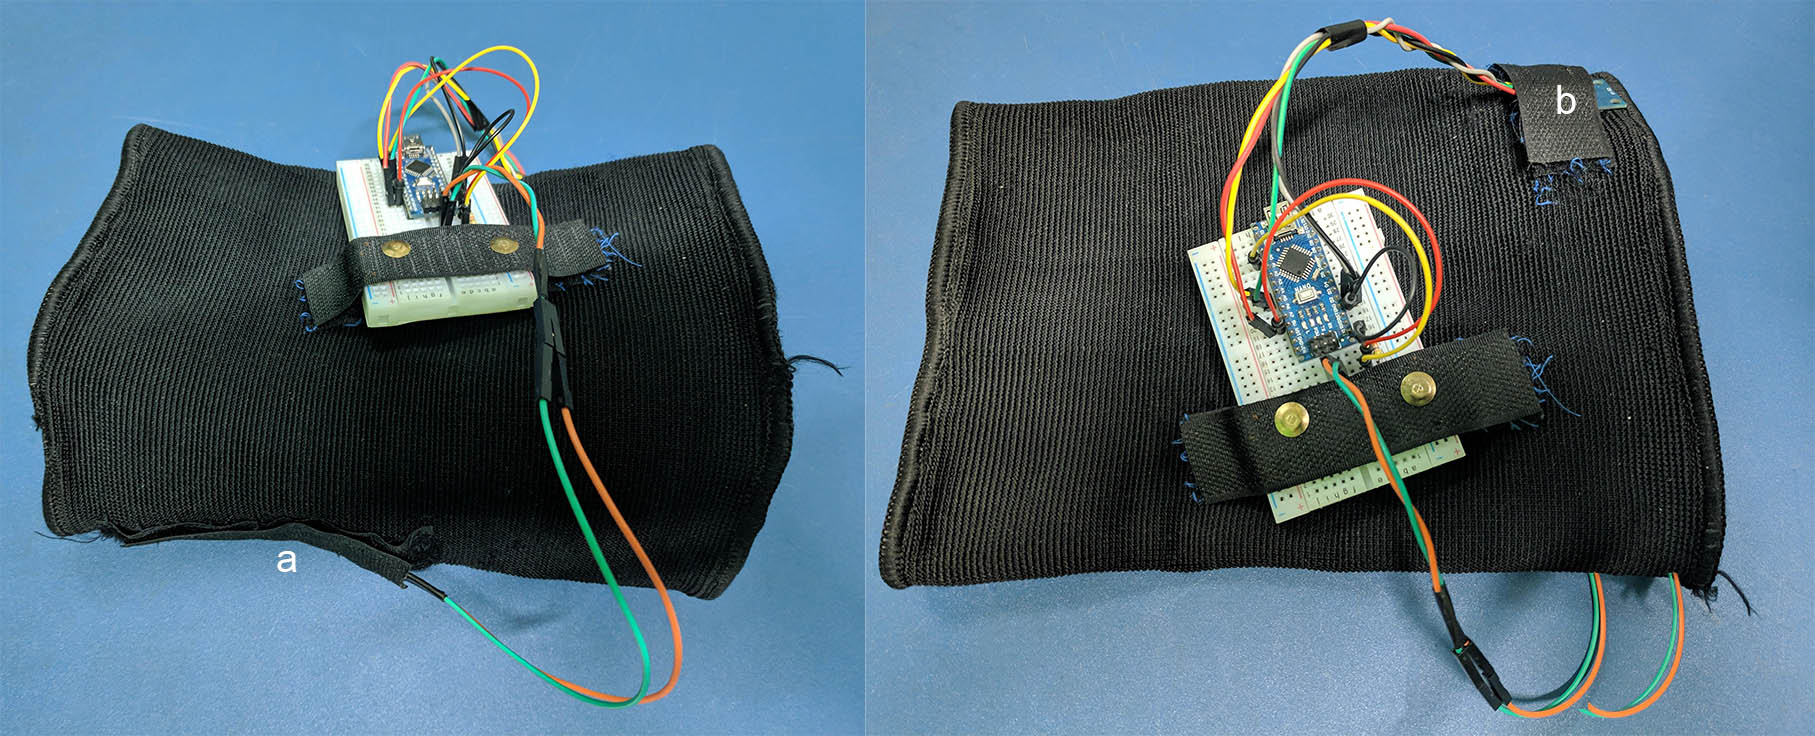
\includegraphics[width=.8\textwidth]{resources/result_prototipo}
	\end{center}
	\legend{Fonte: Elaborada pelo autor}
\end{figure}

Para que fossem feitas a leitura e a classificação dos dados capturados, o Arduino foi conectado via cabo USB em um computador que executava o simulador. Os dados do giroscópio, acelerômetro e resistência do sensor flexível, respectivamente, são enviados continuamente via comunicação serial pelo \textit{software} carregado no Arduino.


% \subsection{\textit{Software} de simulação}\label{sec:result_simulacao}

O sistema de simulação é executado em um computador e foi desenvolvido na linguagem Python $3.7$, para facilitar o uso da ferramenta Scikit-learn\cite{pedregosa:2011}. O programa do simulador é composto por diversos componentes que se integram para realizar diferentes atividades: leitura dos dados, através da biblioteca \textit{pyserial}\footnote{\url{https://github.com/pyserial/pyserial}}; gravação dos dados em arquivos; classificação dos dados, utilizando Scikit-learn; e a exibição $3$D com o uso das bibliotecas \textit{PyOpenGL}\footnote{\url{http://pyopengl.sourceforge.net/}} e \textit{pygame}\footnote{\url{https://www.pygame.org/}}.

%==========================================================================
%
\section{Execução dos experimentos e análise dos resultados}\label{sec:result_execucao}
%
%==========================================================================
Com o protótipo confeccionado e os \textit{softwares} desenvolvidos, deu-se início aos experimentos, visando responder às questões de pesquisa apresentadas na \autoref{sec:result_planejamento} para analisar a eficácia do sistema \productname{} em diferentes cenários de uso.

%---------------------------------------------------------------------------
\subsection{Transmissão de dados e ambiente virtual}
%---------------------------------------------------------------------------

O primeiro experimento realizado, visando responder à primeira questão de pesquisa (\ref{qp:simula_movimentos}), foi focado na transmissão de dados dos sensores para o simulador através da comunicação serial enquanto o ambiente virtual replicava os movimentos realizados pelos sensores.

Os dados de orientação, dentre os que são enviados pelo \textit{software} carregado no Arduino, são recebidos pelo simulador e utilizados como ângulos de rotação do modelo da perna virtual, para replicar a orientação do membro do usuário que está utilizando o protótipo. Durante os experimentos, observou-se que foi necessário fazer uma calibragem do MPU-\(6050\) a partir de sua posição vertical, pois os ângulos de rotação precisam ser relativos a uma posição inicial para que a orientação seja precisa.

Feito isso, o ambiente virtual foi capaz de replicar a posição da perna do usuário, com apenas uma ressalva: a falta de um magnetômetro no MPU\=/6050 utilizado impede que ele realize rotações em torno do eixo perpendicular ao solo, fazendo com que a simulação não reconhecesse bem movimentos de virada. Na \autoref{fig:result_simulacao} é possível ver os valores dos sensores na parte superior, enquanto o modelo virtual os representa graficamente.

\begin{figure}[ht]
	\caption{\label{fig:result_simulacao}Posicionamento da perna virtual conforme dados dos sensores}
	\begin{center}
		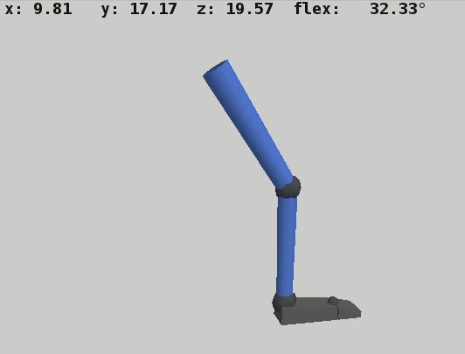
\includegraphics[height=8cm]{resources/result_simulacao}
		%   \missingfigure[figwidth=\textwidth, figheight=5cm]{Fotos lado a lado da simulação e de uma perna usando a joelheira, pra mostrar o modelo 3D funcionando}
	\end{center}
	\legend{Fonte: Elaborada pelo autor}
\end{figure}

%---------------------------------------------------------------------------
\subsection{Classificação de movimentos}\label{sec:result_classif}
%---------------------------------------------------------------------------

Para tornar possível a previsão dos movimentos e para responder à segunda questão de pesquisa (\ref{qp:acuracia}), foi decidido que seriam armazenados os valores do acelerômetro e do sensor flexível, ignorando os dados de orientação do giroscópio, que ainda são utilizados para orientar o modelo virtual. Diversos conjuntos de dados foram gravados com diferentes tipos de ações, como caminhada, subida e descida de degrau.

Todos os dados foram capturados a partir de um cabo USB de \SI{1}{\meter} conectado a um \textit{notebook} (com um processador Intel i7\=/7500U, que conta com \textit{clock} de até \SI{3.5}{\giga\hertz}, e \SI{8}{\giga\byte} de RAM) no sistema operacional Manjaro Linux\footnote{\url{http://manjaro.org/}} 18.0.4, estabelecendo comunicação serial com o programa.

Os indivíduos selecionados para a coleta dos dados tinham os membros intactos e vestiram a joelheira com os equipamentos na perna direita e realizavam as ações necessárias para cada cenário (apresentados nas seções a seguir) do experimento enquanto as transições entre os movimentos eram gravadas em um arquivo.

Após a consolidação do conjunto de dados para cada etapa dos experimentos, foi realizada uma comparação, através de validação cruzada~\cite{scikit:crossval}, entre a acurácia dos diversos algoritmos de classificação disponíveis na ferramenta scikit-learn:
\textit{Logistic Regression}~--~LR~\cite{scikit:lr},
\textit{Linear Discriminant Analysis}~--~LDA~\cite{scikit:lda},
\textit{K\=/Nearest Neighbors}~--~KNN~\cite{scikit:knn},
\textit{CART}~\cite{scikit:cart},
\textit{Gaussian Naive Bayes}~--~NB~\cite{scikit:nb},
\textit{Support Vector Machine}~--~SVM~\cite{scikit:svm},
\textit{AdaBoost Classifier}~--~ADB~\cite{scikit:adb},
\textit{Random Forest Classifier}~--~RFC~\cite{scikit:rfc},
\textit{Extra-Trees Classifier}~--~ETC~\cite{scikit:etc} e
\textit{Gradient Boosting Classifier}~--~GBC~\cite{scikit:gbc}.

%---------------------------------------------------------------------------
\subsubsection{Cenário: caminhada em linha reta}

O primeiro conjunto de dados gerado foi a partir de dois indivíduos que apenas caminhavam em linha reta sobre uma superfície plana. Cada um dos passos de cada perna deveria ser classificado de forma independente. Ou seja, além do estado de repouso (estado \(0\)), foram armazenados o ponto em que a perna esquerda estava para frente (estado \(1\)), e o ponto em que a perna direita estava para frente (estado \(2\)), ilustrados pela \autoref{fig:result_estados}. Ao todo, foram coletadas \(140\) amostras.

\begin{figure}[ht]
	\caption{\label{fig:result_estados}Demonstração das três ações capturadas para a classificação da caminhada}
	\begin{center}
		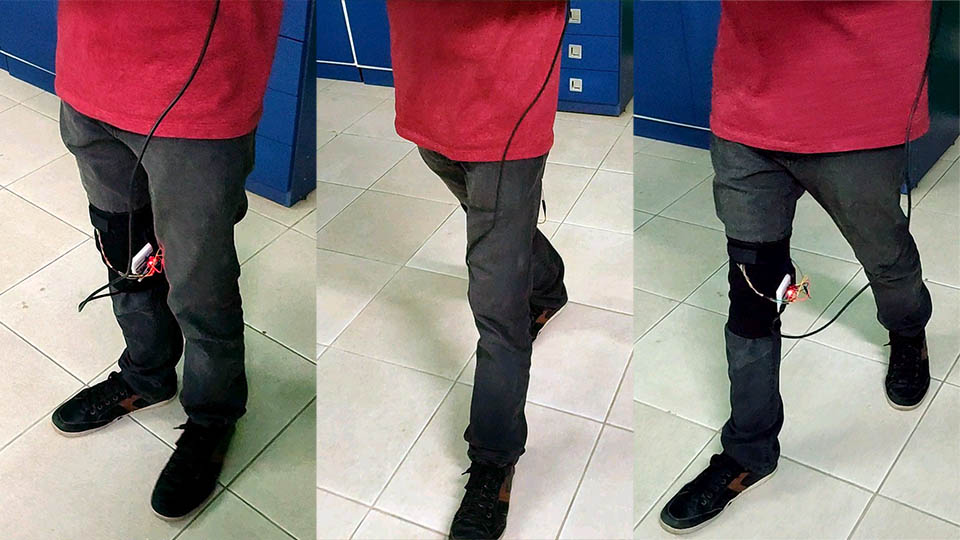
\includegraphics[width=.8\textwidth]{resources/result_estados}
		%\missingfigure[figwidth=\textwidth, figheight=7cm]{Tirar 3 fotos em cada uma das posições para ilustrar as ações no texto (ou só capturar do vídeo de exemplo)}
	\end{center}
	\legend{Fonte: Elaborada pelo autor}
\end{figure}

A partir dos dados coletados dos usuários, verificou-se que \textit{Random Forest} (RFC) seria o algoritmo mais apropriado (\autoref{tab:result_accuracy_rfc}), com acurácia de aproximadamente \(83\%\) para os dados combinados de todos os usuários, como pode ser visto no gráfico da \autoref{fig:result_accuracy_rfc}.

\begin{table}[ht]
	\caption{Comparação dos classificadores com o conjunto de dados combinados para o cenário de caminhada}%
	\label{tab:result_accuracy_rfc}
	\begin{tabularx}{\textwidth}{X X X X X X}
		\toprule
		\textbf{Algoritmo} & LR            & LDA           & KNN           & CART          & NB            \\ \midrule
		\textbf{Acurácia}  & \(50,86\%\)   &   \(69,19\%\)   &   \(62,30\%\)   &   \(75,76\%\)   &   \(69,19\%\) \\ \bottomrule \toprule
		\textbf{Algoritmo} & SVM           & ADB           & RFC           & ETC           & GBC           \\ \midrule
		\textbf{Acurácia}  & \(12,05\%\)   &   \(48,48\%\)   &   \(82,81\%\)   &   \(81,33\%\)   &   \(78,48\%\) \\ \bottomrule
	\end{tabularx}
	\legend{Fonte: Elaborada pelo autor}
\end{table}

\begin{figure}[ht]
	\caption{\label{fig:result_accuracy_rfc}Gráfico de acurácia do classificador \textit{Random Forest} para os dados combinados no cenário de caminhada}
	% 	\todo[inline]{Tentar gerar um gráfico mais interessante: \url{https://scikit-learn.org/stable/auto_examples/model_selection/plot_cv_indices.html}}
	\begin{center}
		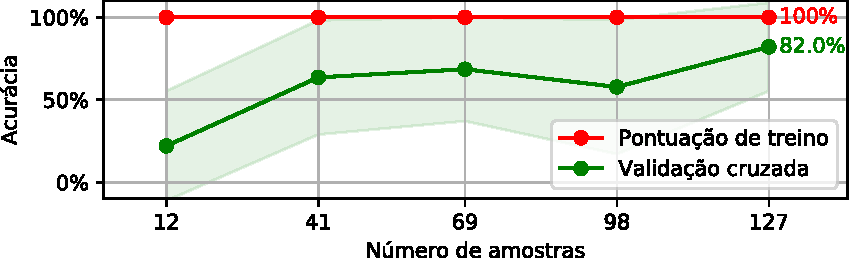
\includegraphics[width=\textwidth]{resources/result_accuracy_rfc}
	\end{center}
	\legend{Fonte: Elaborada pelo autor}
\end{figure}

Ao serem analisados os conjuntos de dados de cada indivíduo, a Análise de Discriminantes Lineares (LDA)~\cite{scikit:lda} obteve maior acurácia, com aproximadamente \(96{,}9\%\), como demonstram a \autoref{tab:result_accuracy_lda} e a \autoref{fig:result_accuracy_lda}. Devido ao pequeno número de amostras, não foi possível gerar um conjunto de dados genérico que funcionasse para todos os indivíduos a partir da coleta realizada. Portanto, uma possível solução seria que cada usuário teria que fazer a própria calibragem do dispositivo para prever os próprios movimentos.

\begin{table}[ht]
	\caption{Comparação dos classificadores com o conjunto de dados individual para o cenário de caminhada}%
	\label{tab:result_accuracy_lda}
	\begin{tabularx}{\textwidth}{X X X X X X}
		\toprule
		\textbf{Algoritmo} & LR            & LDA           & KNN           & CART          & NB            \\ \midrule
		\textbf{Acurácia}  & \(95{,}71\%\) & \(96{,}90\%\) & \(89{,}76\%\) & \(92{,}62\%\) & \(95{,}71\%\) \\ \bottomrule \toprule
		\textbf{Algoritmo} & SVM           & ADB           & RFC           & ETC           & GBC           \\ \midrule
		\textbf{Acurácia}  & \(5{,}00\%\)  & \(94{,}29\%\) & \(94{,}29\%\) & \(94{,}29\%\) & \(91{,}43\%\) \\ \bottomrule
	\end{tabularx}
	\legend{Fonte: Elaborada pelo autor}
\end{table}

\begin{figure}[ht]
	\caption{\label{fig:result_accuracy_lda}Gráfico de acurácia da LDA para um conjunto de dados individual no cenário de caminhada}
	% 	\todo[inline]{Tentar gerar um gráfico mais interessante: \url{https://scikit-learn.org/stable/auto_examples/model_selection/plot_cv_indices.html}}
	\begin{center}
		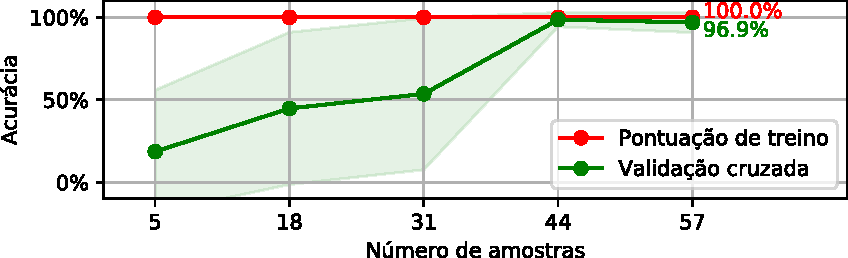
\includegraphics[width=\textwidth]{resources/result_accuracy_lda}
	\end{center}
	\legend{Fonte: Elaborada pelo autor}
\end{figure}

Além disso, ao longo dos experimentos realizados, notou-se que o sensor flexível ficou cada vez menos preciso, o que tornou a visualização $3$D um pouco menos realista, pois o ruído nos dados do sensor tornou-se maior, mas não impediu que os dados fossem classificados e as ações previstas. O uso de um sensor maior, que permitisse seu uso na parte frontal do joelho, pode fazer com que ele se desgaste menos.

%---------------------------------------------------------------------------
\subsubsection{Cenário: Subida e descida de escada}

Após os experimentos com dados de caminhada em linha reta, foram iniciados os experimentos para classificação de subida e descida de degrau. Neste cenário, o usuário deveria subir um degrau com a perna direita (equipada com a joelheira), e descer o degrau com a perna esquerda. Estas ações foram identificadas como \(3\) e \(4\), respectivamente, e estão ilustradas na \autoref{fig:result_poses_degraus}.

\begin{figure}[ht]
	\caption{\label{fig:result_poses_degraus}Ambiente utilizado para coleta de amostras de subida e descida de escada}
	\begin{center}
		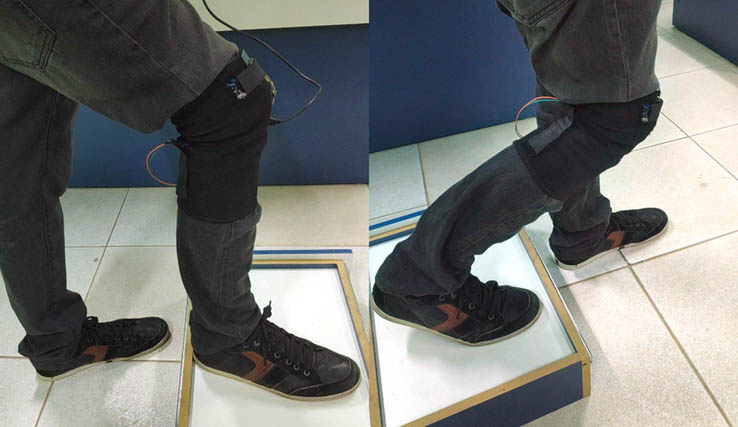
\includegraphics[width=.8\textwidth]{resources/result_poses_degraus}
		%   \missingfigure[figwidth=\textwidth, figheight=5cm]{Fotos das poses de subir e descer degrau}
	\end{center}
	\legend{Fonte: Elaborada pelo autor}
\end{figure}

Ao todo, foram coletadas \(76\) amostras para este cenário. Ao unir ao conjunto de dados de caminhada plana do mesmo usuário, totalizaram-se \(184\) amostras. A comparação dos algoritmos (\autoref{tab:result_accuracy_degraus_1}) resultou com o melhor desempenho do classificador \textit{Gaussian Naive Bayes}. A acurácia deste classificador para os conjuntos de dados combinados foi de apenas \(53\%\), como mostra a \autoref{fig:result_accuracy_degraus_1}.


\begin{table}[ht]
	\caption{Comparação dos classificadores com o conjunto de dados individual para todos os cenários combinados}%
	\label{tab:result_accuracy_degraus_1}
	\begin{tabularx}{\textwidth}{X X X X X X}
		\toprule
		\textbf{Algoritmo} & LR            & LDA           & KNN           & CART          & NB            \\ \midrule
		\textbf{Acurácia}  & \(49{,}44\%\) & \(39{,}82\%\) & \(36{,}20\%\) & \(45{,}03\%\) & \(52{,}43\%\) \\ \bottomrule \toprule
		\textbf{Algoritmo} & SVM           & ADB           & RFC           & ETC           & GBC           \\ \midrule
		\textbf{Acurácia}  & \(04{,}91\%\) & \(22{,}02\%\) & \(46{,}2\%\)  & \(50{,}09\%\) & \(45{,}23\%\) \\ \bottomrule
	\end{tabularx}
	\legend{Fonte: Elaborada pelo autor}
\end{table}


\begin{figure}[ht]
	\caption{\label{fig:result_accuracy_degraus_1}Gráfico de acurácia do classificador \textit{Gaussian Naive Bayes} com o conjunto de dados individual para todos os cenários}
	\begin{center}
		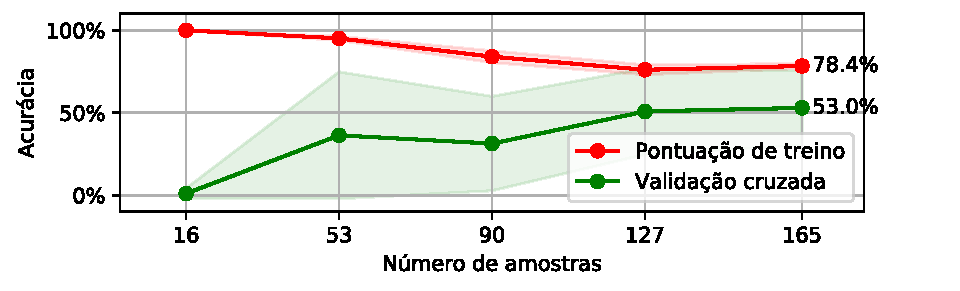
\includegraphics[width=\textwidth]{resources/result_accuracy_degraus_1}
		%   \missingfigure[figwidth=\textwidth, figheight=5cm]{Gráfico de acurácia pro dataset combinado dos dados de repouso e caminhada, junto com o de subir e descer degrau}
	\end{center}
	\legend{Fonte: Elaborada pelo autor}
\end{figure}
\newpage
Em seguida, portanto, foram realizados testes com apenas os dados capturados para este cenário, removendo da classificação os dados gerados no cenário de caminhada. Neste caso, o algoritmo com melhor desempenho, conforme a \autoref{tab:result_accuracy_degraus_2}, foi o \textit{Extra-Trees}, com \(84{,}5\%\) de acurácia, como visto no gráfico da \autoref{fig:result_accuracy_degraus_2}.

\begin{table}[ht]
	\caption{Comparação dos classificadores com o conjunto de dados individual para o cenário de subida e descida de degrau}%
	\label{tab:result_accuracy_degraus_2}
	\begin{tabularx}{\textwidth}{X X X X X X}
		\toprule
		\textbf{Algoritmo} & LR            & LDA           & KNN           & CART          & NB            \\ \midrule
		\textbf{Acurácia}  & \(63{,}93\%\) & \(71{,}96\%\) & \(67{,}68\%\) & \(80{,}54\%\) & \(70{,}71\%\) \\ \bottomrule \toprule
		\textbf{Algoritmo} & SVM           & ADB           & RFC           & ETC           & GBC           \\ \midrule
		\textbf{Acurácia}  & \(26{,}79\%\) & \(30{,}54\%\) & \(80{,}36\%\) & \(81{,}96\%\) & \(67{,}50\%\) \\ \bottomrule
	\end{tabularx}
	\legend{Fonte: Elaborada pelo autor}
\end{table}

\begin{figure}[ht]
	\caption{\label{fig:result_accuracy_degraus_2}Gráfico de acurácia do classificador \textit{Extra-Trees} com o conjunto de dados individual para o cenário de subida e descida de degrau}
	\begin{center}
		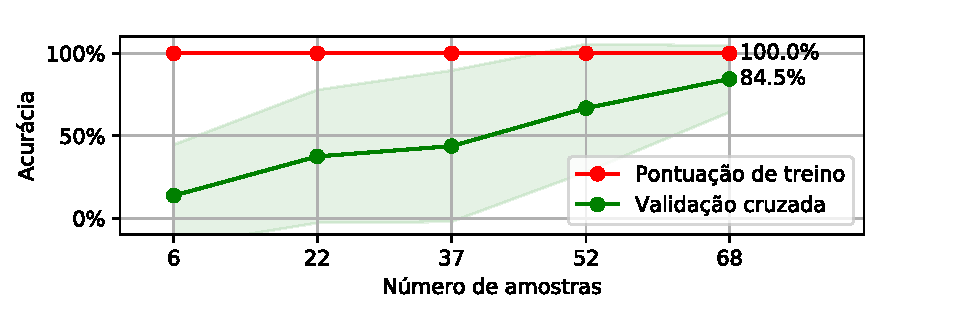
\includegraphics[width=\textwidth]{resources/result_accuracy_degraus_2}
		%   \missingfigure[figwidth=\textwidth, figheight=6cm]{Gráfico de acurácia pro dataset isolado só com os dados gerados no dia do degrau}
	\end{center}
	\legend{Fonte: Elaborada pelo autor}
\end{figure}

Em vista destes resultados, constata-se que quanto maior o número de classes, maior é o número de amostras necessárias para o classificador e no caso de ter a disponibilidade de um número maior de amostras, o sistema deve conseguir funcionar de forma mais precisa com diversos tipos de cenários.

%---------------------------------------------------------------------------
\subsection{Simulação da prótese em tempo real}
%---------------------------------------------------------------------------

Por fim, com o intuito de responder à terceira questão de pesquisa (\ref{qp:previsao_sensores}), a animação da prótese virtual foi avaliada em relação à confiabilidade da ação de seus atuadores. Utilizando apenas o conjunto de dados correspondente ao usuário que estava vestindo o dispositivo, observou-se a ativação da prótese, conforme o usuário caminhava em linha reta.

\begin{figure}[ht]
	\caption{\label{fig:result_simulacao_atuadores}Simulação dos atuadores da prótese a partir da classificação dos dados dos sensores}
	\begin{center}
		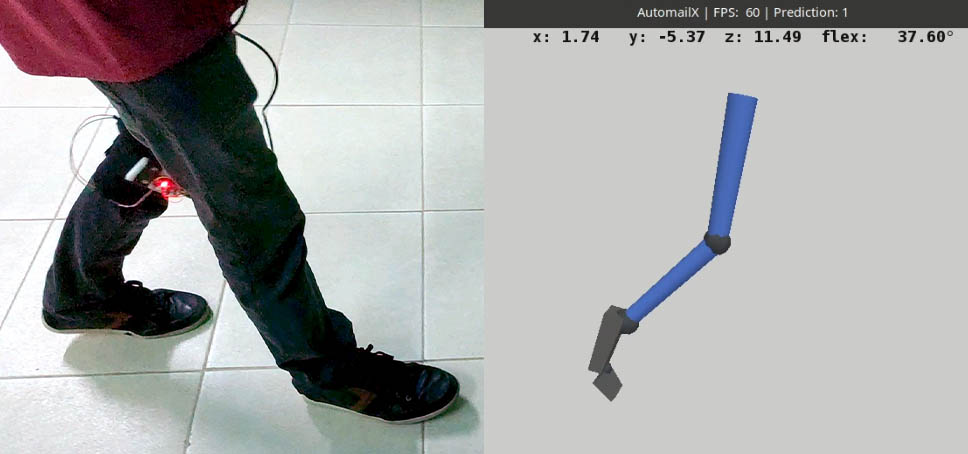
\includegraphics[width=\textwidth]{resources/result_simulacao_atuadores}
	\end{center}
	\legend{Fonte: Elaborada pelo autor}
\end{figure}

A simulação animada em 3D mostrou-se capaz de exibir o movimento realizado pelos dois sensores em tempo real e, além da ação realizada na prótese simulada. A \autoref{fig:result_simulacao_atuadores} mostra a ação correspondente a um passo com a perna oposta à perna com os sensores, ativando os atuadores da prótese ao detectar a classe \(1\).

Neste experimento de caminhada, de \(8\) passos realizados com a perna direita, apenas \(2\) não foram reconhecidos corretamente, enquanto todos os \(8\) passos realizados com a perna esquerda (\autoref{fig:result_simulacao_atuadores}) e o estado de repouso foram classificados corretamente.